\documentclass[11pt]{report}
\usepackage{amsmath}
\usepackage{amssymb}
\usepackage{amsfonts}
\usepackage{mathtools}
\usepackage{amsthm}
\usepackage{ragged2e}
\usepackage[hidelinks]{hyperref}
\usepackage{float}
\usepackage{pgf,tikz}
\usepackage[shortlabels]{enumitem}
\usepackage{color}
\usepackage{pgfplots}
\usepackage[margin = 1 in]{geometry}
\usepackage{mathrsfs}
\usetikzlibrary{arrows}
\usepackage{multicol}
\usepackage{fancyhdr}
\pagestyle{fancy}
\usepackage{multirow}
\usepackage{graphicx}
\usepackage{psfrag}
\usepackage{biblatex}
\addbibresource{hw8.bib}
\usepackage{listings}
\renewcommand{\footrulewidth}{0.4pt}

\newtheorem{theorem}{Theorem}[chapter]
\newtheorem{defn}{Definition}[chapter]
\newtheorem{lemma}{Lemma}[chapter]

\theoremstyle{definition}
\newtheorem{proposition}{Proposition}[chapter]
\newtheorem{remark}{Remark}[chapter]
\newtheorem{example}{Example}[chapter]

\DeclareMathOperator*{\argmin}{arg\,min}
\DeclareMathOperator*{\argmax}{arg\,max}

\newcommand{\user}{}
\newcommand{\xlr}[2]{#1 \left(#2\right)}
\newcommand{\clr}[2]{#1 \left\{ #2 \right\}}
\newcommand{\rank}{\mathrm{rank}}
\newcommand{\mat}[1]{\mathbf{#1}}
\lhead{ECE 530 - Fall 2023 at University of Illinois at Urbana-Champaign}
\rhead{HW8}
\lfoot{Author: \textcolor{red}{Eric Silk, esilk2}}
\rfoot{Due: Fri. November 17}
\begin{document}


\section*{Problem 1: Appreciate Cholesky Graphically}
\subsection*{Problem Statement}
\begin{figure}[h]
	\center
	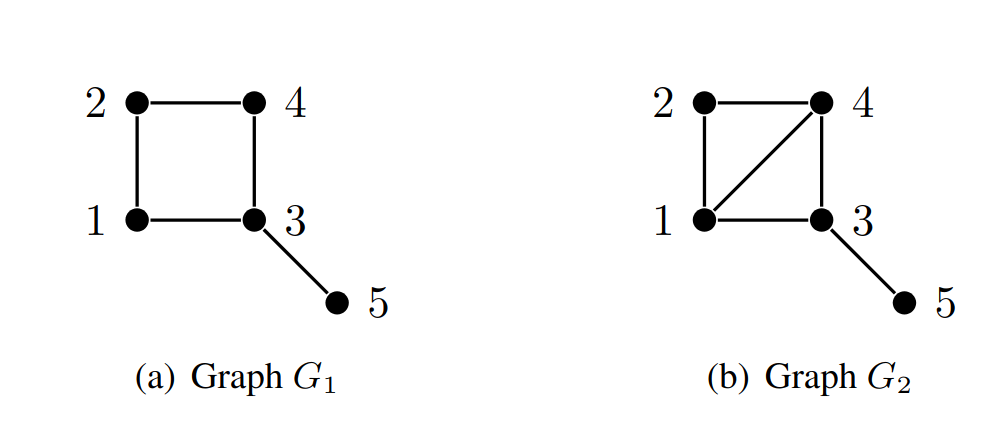
\includegraphics[width=.8\textwidth]{graph_fig.png}
\end{figure}

\subsubsection*{a}
Find a matrix $\mat{A}\in\mathbb{R}^{5\times5}$ s.t $\mathcal{G}(\mat{A})=G_1$ in the figure
above, and s.t. $\mat{A}\succ0$.
\textit{Hint: Associate positive numbers or weights to each node and each edge
of $G_1$. Define $A_{ij}=A_{ji}$ as the negative of the weight on the edge
$(i,j)$ of $G_1$. Define $A_{ii}$ to be the sum of the weight of node $i$ and the
weights of all edges connected to node $i$. Such a matrix is called a Laplacian
matrix for $G_1$. Compute the eigenvalues to verify it is indeed PD.}

\subsubsection*{b}
Compute the lower triangular Cholesky factor $\mat{L}\in\mathbb{R}^{5\times5}$
with positive diagonals such that $\mat{L}\mat{L}^T$ equals $\mat{A}$ in part
(a). Draw a graph on 5 nodes that describes the sparsity pattern of $\mat{L}$;
i.e. draw $G(\mat{L})$. Verify that $G(\mat{L})$ is a chordal graph.

\subsubsection*{c}
Notice that $G_2$ in figure 1b is a chordal graph. Find a permutation matrix
$\mat{P}$ s.t. that when you compute the Cholesky factor $\mat{L}'$ of
$\mat{PAP}^T$ with your $\mat{A}$ from part (a), then $G(\mat{L}')=G_2$.
\textit{Hint: Eliminate the nodes of $G_1$ in the sequence $(5,2,3,1,4)$. Encode
	that elimination order in a permutation matrix.}

\subsubsection*{d(**)}
Let $\mat{X}\in\mathbb{R}^{n\times n}$ be a PD matrix and
$\mat{\Gamma}\in\mathbb{R}^{n\times n}$ be a lower triangular matrix with
positive diagonals, s.t. $\mat{X}=\mat{\Gamma\Gamma}^T$. Prove that $G(\mat{X})$
is a subgraph of $G(\mat{\Gamma})$ and $G(\mat{\Gamma})$ is a chordal graph.
\textit{Hint: Use an induction argument on the size of the matrix. Characterize
	how the steps in Cholesky factorization shapes the sparsity pattern of
	$\mat{\Gamma}$. Finally, utilize the fact that if a node and a set of edges from
	that node is added to a chordal graph $G$, then the obtained graph is chordal
	IFF every two neighbors of the new node in $G$ already shared an edge in $G$.}

\subsection*{Solution}
For script, see relevant section at the end of the document.

\subsubsection*{a}
Relevant script output:
\begin{lstlisting}[basicstyle=\small]
1a Laplacian:
[[ 3. -1. -1.  0.  0.]
[-1.  3.  0. -1.  0.]
[-1.  0.  4. -1. -1.]
[ 0. -1. -1.  3.  0.]
[ 0.  0. -1.  0.  2.]]
1a eigenvalues:
[5.481 1.    1.83  3.    3.689]
1a PD: True
\end{lstlisting}
\begin{figure}[H]
	\center
	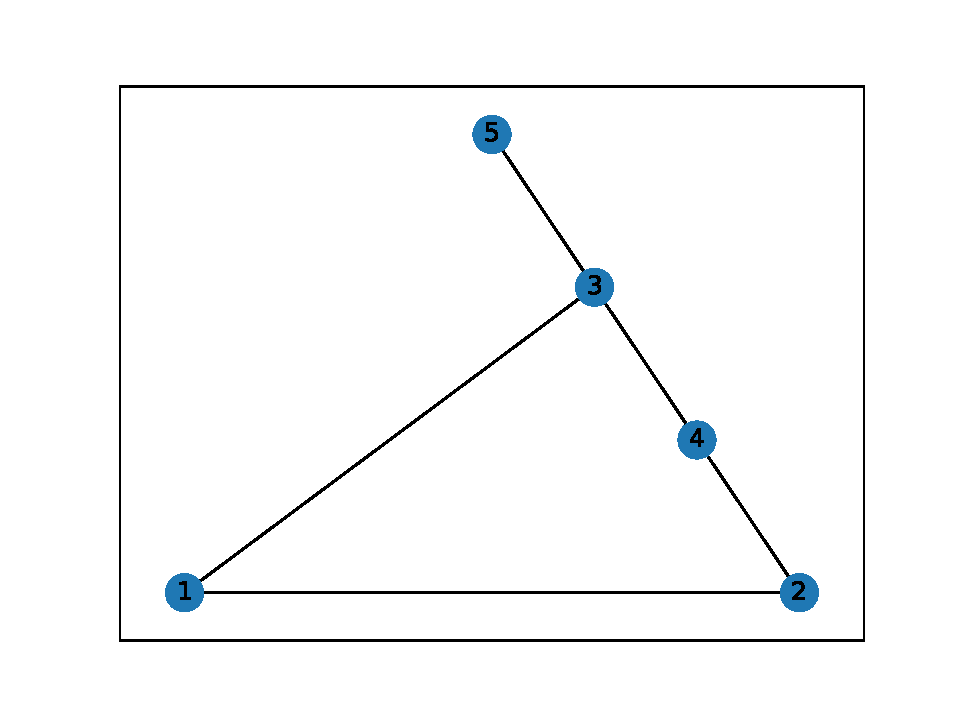
\includegraphics[width=.8\textwidth]{one_a.pdf}
	\caption{Graph $G_1$ generated in networkx, for verification}
\end{figure}

\subsubsection*{b}
\begin{lstlisting}[basicstyle=\small]
1b L:
[[ 1.732  0.     0.     0.     0.   ]
 [-0.577  1.633  0.     0.     0.   ]
 [-0.577 -0.204  1.904  0.     0.   ]
 [ 0.    -0.612 -0.591  1.509  0.   ]
 [ 0.     0.    -0.525 -0.206  1.297]]
\end{lstlisting}
\begin{figure}[H]
	\center
	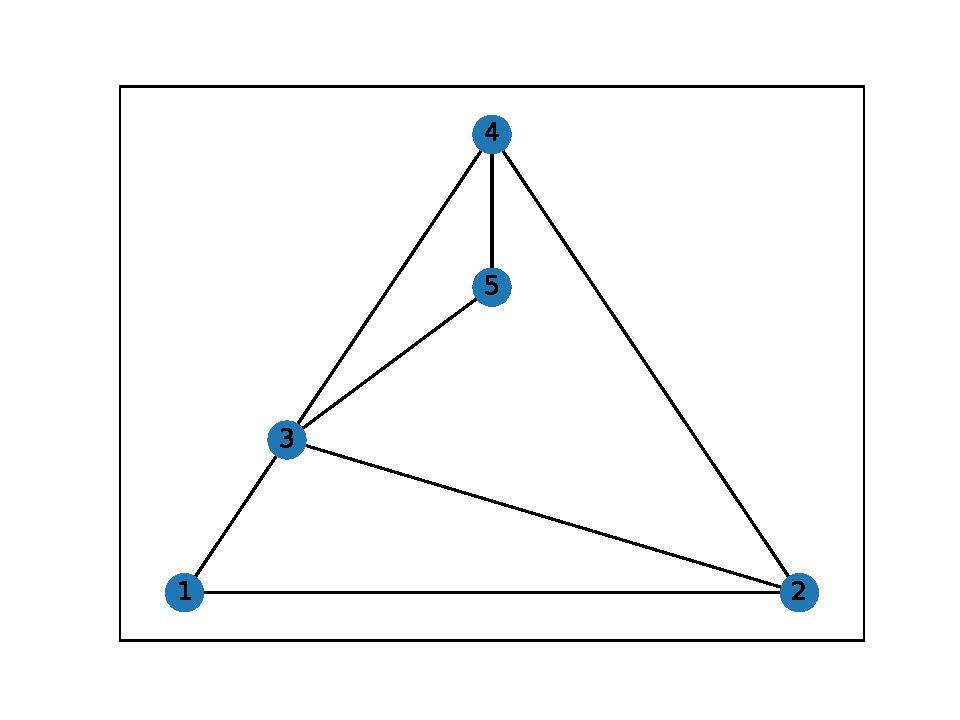
\includegraphics[width=.8\textwidth]{one_b.pdf}
	\caption{Graph $\mathcal{G}(L)$ generated in networkx. Note it is indeed chordal.}
\end{figure}

\subsubsection*{c}
\begin{figure}[H]
	\center
	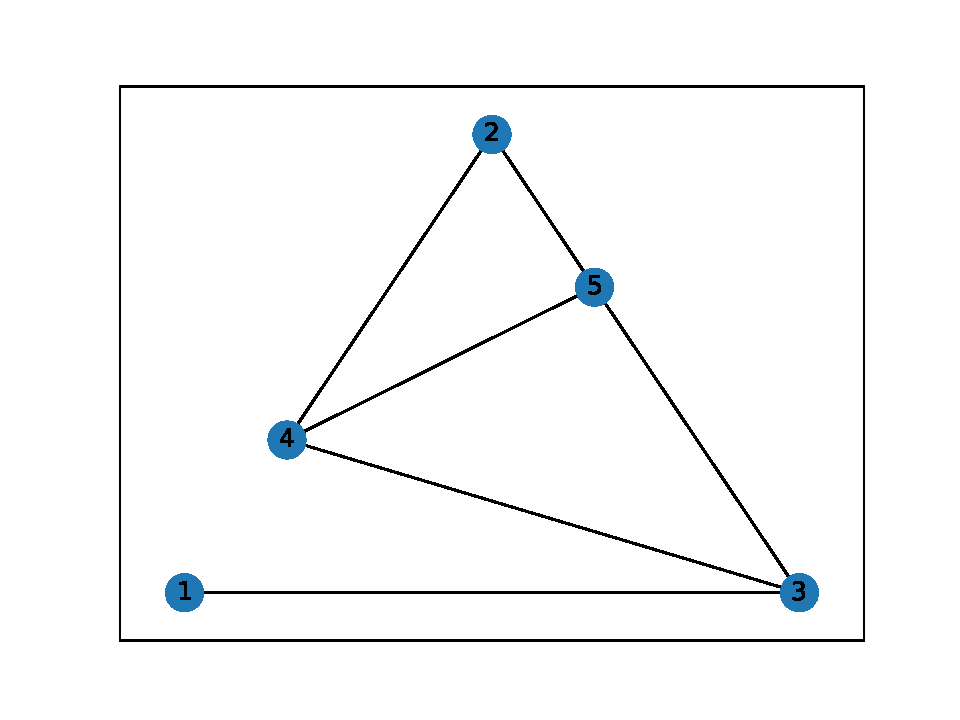
\includegraphics[width=.8\textwidth]{one_c.pdf}
	\caption{Graph $\mathcal{G}(L')$ generated in networkx. Note it indeed
		matches the structure of $G_2$ with the nodes swapped as described.}
\end{figure}

\subsubsection*{d}
...meh, it's 4PM on the Friday before break.

\newpage

\section*{Problem 2: Split 'em matrices for Linear Systems}
\subsection*{Problem Statement}
Consider a linear system of equations $Ax=b$ where $A\in\mathbb{R}^{n\times n}$
and $\exists A^{-1}$. The matrix splitting method splits $A$ as $A=M-n$ and
successively solves the equation:
\begin{equation}
	x^{k+1}=M^{-1}\left(Nx^k+b\right)
\end{equation}
for $k\geq 0$ to perform a fixed-point iteration in order to solve the linear system $Ax=b$. Identify $L,D$ and $U$ as the strictly lower triangular, diagonal, and strictly upper triangular part of $A$. Then, $A=L+D+U$. Whem $M=L+D$, then the fixed point iteration becomes:
\begin{equation}
	x_i^{k+1}\coloneqq \frac{1}{A_{ii}}\left[
	b_i - \sum_{j<i}A_{ij}x_{j}^{k+1}-\sum_{j>i}A_{ij}x_j^k
	\right]
\end{equation}
for $i=1,\ldots,n$ and $k\geq 0$.
\subsubsection*{a}
Write the update equation for each element of $x$ as in equation 2 when $M=D+U$ using
backward induction to compute the iterates in equation 1 successively.

\subsubsection*{b}
Call the method you devised in part (a) as the \textit{backward} Gauss-Seidel
method. Which among this method and Jacobi methods would you expect to converge
faster to the solution of $Ax=b$? Which one will you choose if distributed
computation is involved, and why?

\subsubsection*{c}
Implement both backward Gauss-Seidel and Jacobi methods to solve the linear system of equations
$Ax=b$ with
\[
	A\coloneqq \begin{pmatrix}
		10 & 5  & 3 & 4 \\
		4  & 10 & 2 & 1 \\
		1  & 3  & 8 & 2 \\
		1  & 6  & 3 & 9
	\end{pmatrix},\
	b\coloneqq \begin{pmatrix}
		4 \\ -5 \\ 4 \\ -11
	\end{pmatrix}
\]
starting with $x^0\coloneqq (1,1,1,1)^T$. Plot the residues and errors in the
succesive iterates on a semilog plot. Iterate until the residue falls below $10^-5$. The error and residue, respectively, at iteration $k$ are given by:
\[ \epsilon^k\coloneqq \|x-x^*\|,\ r^k\coloneqq \|b-Ax^k\| \]
where $x^*$ is the solution to the linear system.

\subsubsection*{d}
Recall that the method of succesive over-relaxation (SOR) uses
$M=\frac{1}{\omega}D+L$. Any matrix splitting method converges to the solution
of a linear system \textit{IF} the spectral radius of the matrix $I-M^{-1}A$ is
less than 1. Plot the spectral radius of $I-M^{-1}A$ for SOR as a function of
$\omega$ in the range $[0.01, 2.20]$ for 20 randomly generated PD $A$ matrices
on the same graph. Based on your plot, can you guess for what values of $\omega$
SOR converges for PD matrices?


\subsection*{Solution}
\subsubsection*{a}
\[
	x_i^{k+1}\coloneqq \frac{1}{A_{ii}}\left[
	b_i - \sum_{j>i}A_{ij}x_{j}^{k+1}-\sum_{j<i}A_{ij}x_j^k
	\right]
\]

\subsubsection*{b}
It will depend. Gauss-Seidel methods use more ``up to date'' information, and so intuitively we would expect faster convergence. However,
this is not a hard and fast rule, and there are counterexamples wherein one method converges and the other doesn't, OR that one will converge faster in certain cases, or slower in others.
See \cite{Venit_1975}.

I think that using a typical scatter-gather scheme for distributed computation,
Jacobi iteration would be preferred for distributed computing. Each element of
$x^{k+1}$ can be calculated in an embarrasingly parallel fashion (i.e. each
element can be calculated in a fully independent fashion), whereas Gauss-Seidel
will require iterations and sharing current estimates of $x^{k+1}$ around, which
will limit the ability to parallelize.

\subsubsection*{c}
\begin{figure}[H]
	\center
	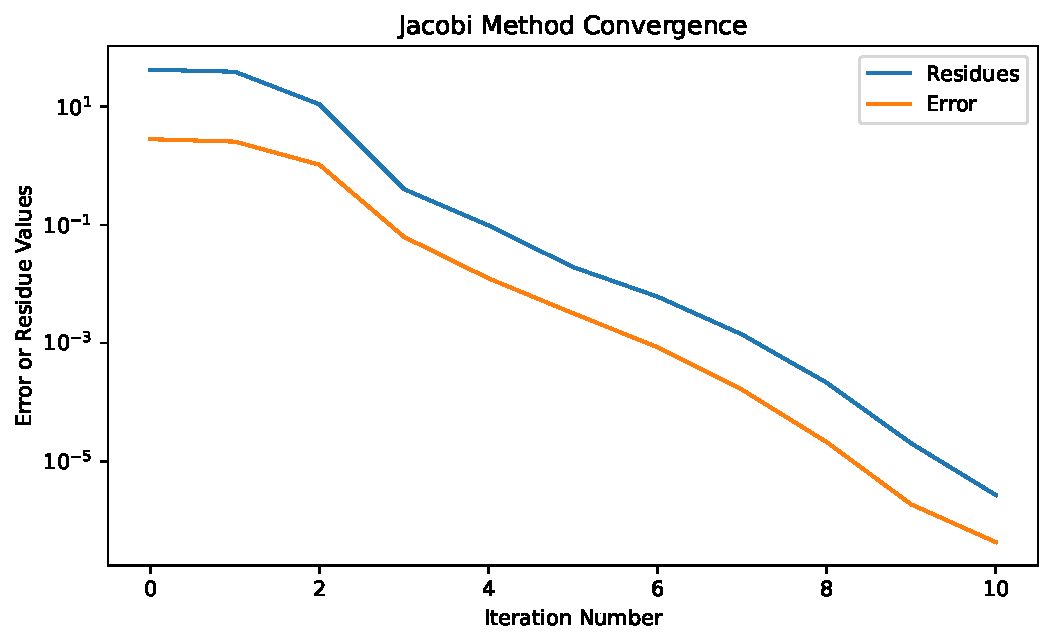
\includegraphics[width=.8\textwidth]{jacobi_iter.pdf}
\end{figure}
\begin{figure}[H]
	\center
	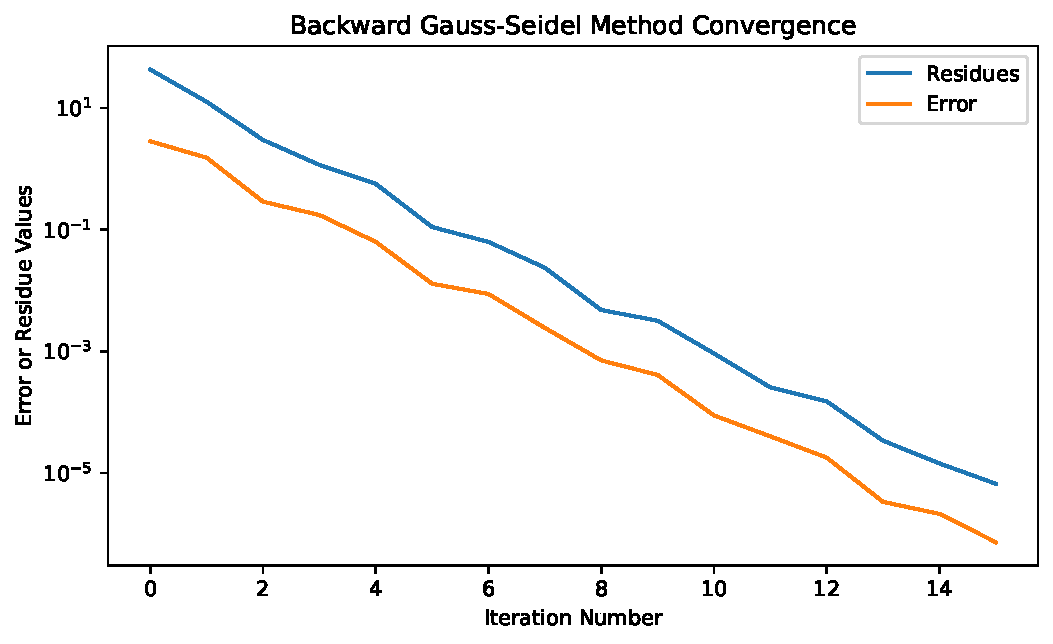
\includegraphics[width=.8\textwidth]{bgs_iter.pdf}
\end{figure}


\subsubsection*{d}
\begin{figure}[H]
	\center
	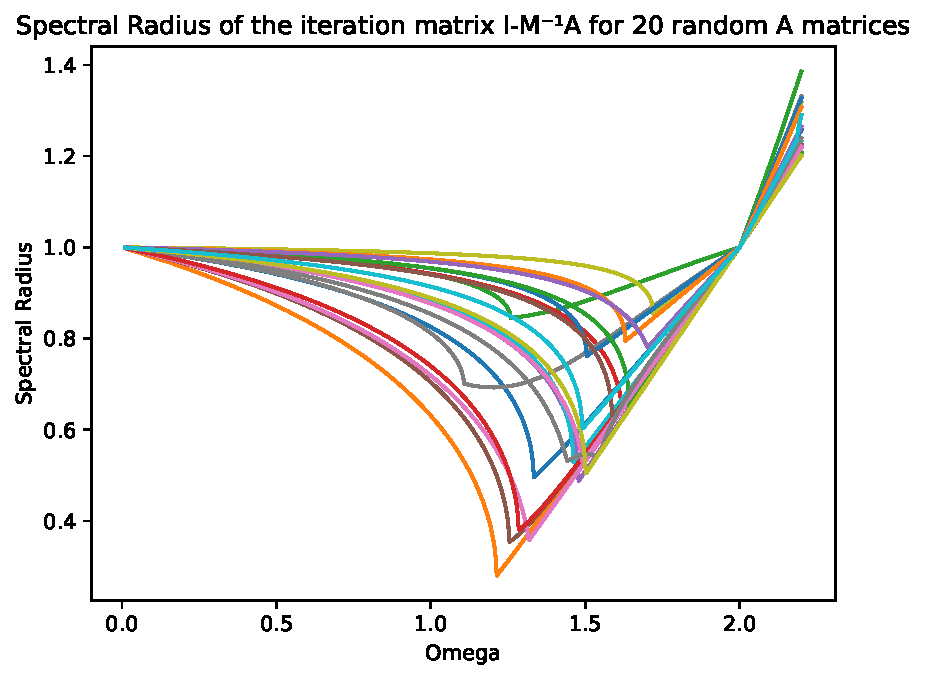
\includegraphics[width=.8\textwidth]{sor_omegas.pdf}
\end{figure}
Empirically it appears that the spectral radius will be less than 1 for values
between 0 and 2.  This is in fact a proven property of SOR methods, according to
the Wikipedia article on them.

\newpage
\section*{Code}
\definecolor{codegreen}{rgb}{0,0.6,0}
\definecolor{codegray}{rgb}{0.5,0.5,0.5}
\definecolor{codepurple}{rgb}{0.58,0,0.82}
\definecolor{backcolour}{rgb}{0.95,0.95,0.92}
\lstdefinestyle{mystyle}{
	backgroundcolor=\color{backcolour},
	commentstyle=\color{codegreen},
	keywordstyle=\color{magenta},
	numberstyle=\tiny\color{codegray},
	stringstyle=\color{codepurple},
	basicstyle=\ttfamily\footnotesize,
	breakatwhitespace=false,
	breaklines=true,
	captionpos=b,
	keepspaces=true,
	numbers=left,
	numbersep=5pt,
	showspaces=false,
	showstringspaces=false,
	showtabs=false,
	tabsize=2
}
\lstset{style=mystyle}


\subsection*{Problem 1}
\lstinputlisting[
	language=Python,
	basicstyle=\tiny
]{../../ece530/ece530/hw8/problem1.py}
\newpage
\subsection*{Problem 2}
\lstinputlisting[
	language=Python,
	basicstyle=\tiny
]{../../ece530/ece530/hw8/problem2.py}
\printbibliography
\end{document}
